% template created by: Russell Haering. arr. Joseph Crop
\documentclass[12pt,letterpaper]{article}
\usepackage{anysize}
\usepackage{cite}
\usepackage{amsmath,amssymb,amsfonts}
\usepackage{algorithm}
\usepackage[noend]{algpseudocode}
\usepackage{graphicx}
\usepackage{multirow}
\usepackage{listings}
\usepackage{xcolor}


\marginsize{2cm}{2cm}{1cm}{1cm}

\lstset{ framexleftmargin=9mm, frame=shadowbox,tabsize = 4}

\begin{document}

\begin{titlepage}
    \vspace*{4cm}
    \begin{flushright}
    {\huge
        ECE 375 Lab 3\\[1cm]
    }
    {\large
       Data Manipulation and the LCD
    }
    \end{flushright}
    \begin{flushleft}
    Lab session: 015
    
    Time: 12:00-13:50
    \end{flushleft}
    \begin{flushright}
    Author: Astrid Delestine

    Programming partner: Lucas Plastid 

    \vfill
    \rule{5in}{.5mm}\\
    TA Signature
    \end{flushright}

\end{titlepage}

\section{Introduction}
%This is the first Lab in the ECE 375 series and it covers the setup and compilation of an AVR Assembly Program. The student will learn how how to use the sample Basic Bump Bot assembly file and send the binaries to the AVR Microcontroller board. For the second part of the lab the student will be expected to download and compile the included C sample program and from it learn how to configure the I/O ports of the ATmega32U4 Microcontroller. The student will then write their own C program and upload it to the Microcontroller to verify that it runs as expected. The provided programs have been attached in the source code section of this report.
This is the third lab in the ECE 375 series and it covers a basic introduction to the connected LCD panel, and introduces the idea of peripherals to the student. Additionally it also covers data manipulation, in the different data spaces. The students job for this lab is to use the given LCD Driver to do 3 different things, Firstly clear the display of any static or previous data, Secondly, statically print the names of the two team members to the LCD, and finally, have the LCD operate in a marquee fashion, rotating the text to the right. 

\section{Design}
To design the program for this lab, Lucas and I brainstormed exactly what needed to happen and how we wanted it to go. We needed to determine what the buttons were going to do, and so with the main guide's and the presentation slides, we planned to have four different buttons clear the display, set the display to static text, scroll through the display in a marquee fashion and halt the marquee function when needed. Below one can see a block diagram of what our original plan was.

\begin{figure}[h]
	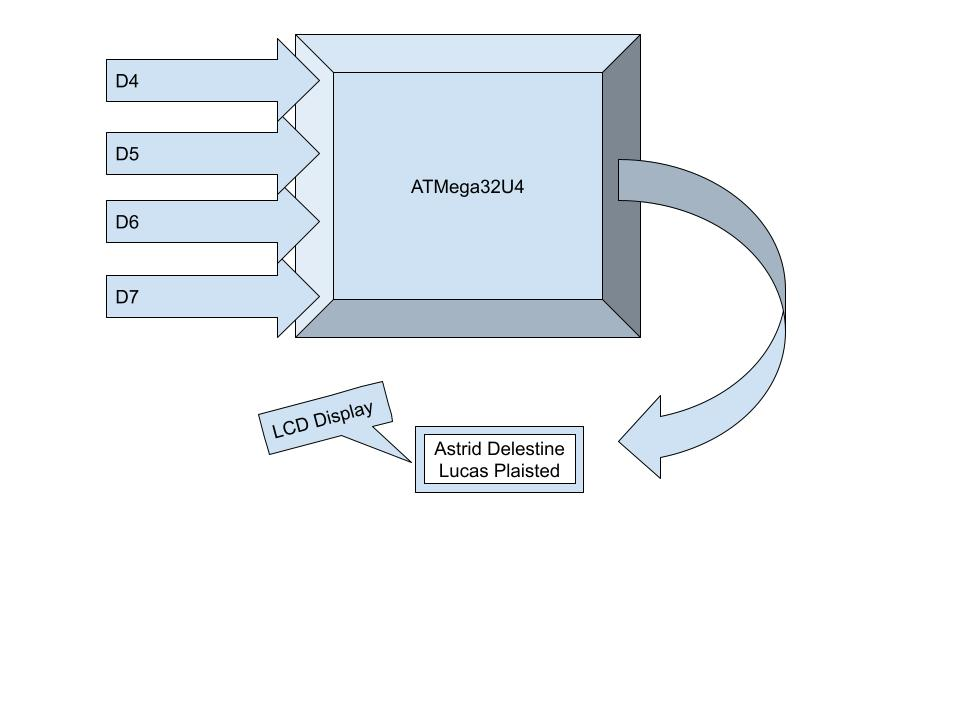
\includegraphics[width=12cm, height=10cm]{BlockDiagramLab3.jpg}
	\centering
\end{figure}
	
\section{Assembly Overview}
As for the Assembly program an overview can be seen below

\subsection{Internal Register Definitions and Constants}
The multipurpose register was setup as r16. a wait counter register was setup at r17. For the timer function an inner counter and outer counter register were setup as r18 and r19 respectively. Several different values of importance were also named such as the LCD memory locations for the first line, the second line, and the end of the second line. 

\subsection{Initialization Routine}
Firstly the stack pointer is initialized, next the LCD display is initialized via an rcall. Finally the port D is initialized to have all inputs. 

\subsection{Main Routine}
The main routine is quite simple, First a function is called BTN2MPR, then using the output of this function, expected to be saved to mpr, we can compare particular bits to see if buttons have been pressed. If a button, say button d5 is pressed, then an rcall is made to DISPNAMES. This will continue to loop until the end of time. 


\subsection{Subroutines}
	\subsection{MARQUEE}
	The marquee function will shift letters from their current locations to the right and if they go off the screen they will loop around. This will happen at a stock rate of 1 movement per quarter second. This can be adjusted. Marquee will continue until button 6 is pressed. First the function loads the display with all the characters then it goes into its main loop, rotating the characters back and forth, and making sure to write to the LCD in between each moment. Some added functionality of this subroutine is that we can speed up or slow down the marquee if necessary. Once button 6 has been pressed the loop will end and the function returns to the main or wherever called it. 
	
	\subsection{ROTCHAR}
	ROTCHAR rotates all charters right through the memory where the LCD pulls from. It does not write to the display it only edits the memory locations. It preforms this action by pushing the variables it is going to use to the stack for safe keeping, then it loads the LCD Ends into the Y pointer. It then pulls the last character and saves it into mpr and pushes it to the stack. Mpr is then loaded with the pre-decremented location of Y, causing the letter before last to be saved into mpr. it is then moved up by 1 in memory, and this will continue until the first character is moved, then the loop breaks and the first character is set to the character previously pushed to the stack. Finally all variables are popped back to their previous locations and the program counter returns to where it was before.  


	\subsubsection{BTN2MPR}
	Places the 4 button inputs into the higher 4 bits of mpr. These buttons are active low. To confirm that it is only the 4 top most bits being saved into mpr an and filter is applied before returning to the main function. 
	
	\subsubsection{DISPNAMES}
	This subroutine is quite simple, it first pushes all the variables it is going to use onto the stack. Then it loads the string locations into the Z pointer, it also loads the LCD locations into the Y pointer. Then using mpr it copies data from the Z pointer to the LCD location 1 letter at a time, until both the top and the bottom buffers have been filled. then it calls the lcd write function, and finally pops all the saved variables off the stack before returning back to the previous function. 
	
	\subsubsection{Wait}
	The Wait subroutine controls the wait intervals while another function is preforming an action. Due to each clock cycle taking a measurable amount of time, we can calculate how many times we need to loop for. This function used the olcnt and ilcnt to have two nested loops, running the dec command until they equal zero, thus waiting the requested amount of time. \textbf{The original program was changed by modifying the Wtime constant value by shifting the bit back by 1 space inside of the HitRight subroutine and the HitLeft subroutine. This effectively doubles the wait time. See Lines 167, 201}


\section{Testing}
Tested each button
\begin{table}[h]
	\centering
	\begin{tabular}{|l|l|l|ll}
		\cline{1-3}
		Case & Expected & Actual meet expected &  &  \\ \cline{1-3}
	D4 Pressed	&Clears the Display&	\checkmark  &  \\ \cline{1-3}
	D5 Pressed	&Shows 2 lines of text, Each name&	\checkmark	&  \\ \cline{1-3}
	D6 Held after D7 is Pressed	&Cancels Marquee&	\checkmark  &  \\ \cline{1-3}
	D7 Pressed	&Begins Marquee&	\checkmark	&  \\ \cline{1-3}
	
%		&          &                      &  &  \\ \cline{1-3}
	\end{tabular}
\caption{Assembly Testing Cases}
\end{table}

\section{Additional Questions}
\begin{enumerate}
    \item
    In this lab, you were required to move data between two memory types: program memory and data memory. Explain the intended uses and key differences of these two memory types.

    The intended use of data memory is to store large amounts of data that is persistent on reboot. Program memory is filled on the fly and is considered more versatile. It is however cleared without power. 

	\item 
	You also learned how to make function calls. Explain how making a function call works (including its connection to the stack), and explain why a RET instruction must be used to return from a function. 
	
	Function calls (rcall) are used to jump to an external to the main function, function. This allows for a cleaner, and easier to read program, that could be more efficient. One important factor of the rcall function is that the program counter is pushed to the stack when it is called, so it is very important to have the stack pointer initialized, and once a function is complete it must end with a ret call, to return to the main function, or to wherever the program counter was last.
	
	
	\item 
	Write pseudocode for an 8-bit AVR function that will take two 16-bit numbers (from data memory addresses \$0111:\$0110 and \$0121:\$0120), add them together, and then store the 16-bit result (in data memory addresses \$0101:\$0100). (Note The syntax “\$0111:\$0110” is meant to specify that the function will expect little-endian data, where the highest byte of a multi-byte value is stored in the highest address of its range of addresses.)
	
	ldi XH, \$01 \newline
	ldi XL, \$10 \newline
	ldi YH, \$01 \newline
	ldi YL, \$20 \newline
	ldi ZH, \$01 \newline
	ldi ZL, \$00 \newline
	CLR Z
	ADW Z+1:Z Y+1:Y //add word
	ADW Z+1:Z X+1:X // add word
	
	
	\item 
	Write pseudocode for an 8-bit AVR function that will take the 16-bit number in \$0111:\$0110, subtract it from the 16-bit number in \$0121:\$0120, and then store the 16-bit result into \$0101:\$0100

	ldi XH, \$01 \newline
	ldi XL, \$10 \newline
	ldi YH, \$01 \newline
	ldi YL, \$20 \newline
	ldi ZH, \$01 \newline
	ldi ZL, \$00 \newline
	CLR Z
	SUW Z+1:Z Y+1:Y //subtract word
	SUW Z+1:Z X+1:X //subtract word

    
	

\end{enumerate}

\section{Difficulties}
This lab was not too difficult, however determining exactly how the marquee needed to work was definitely a challenge. After sorting out the bugs, it was extremely exciting to see text show up on the display.  

\section{Conclusion}
This lab really helped teach just how peripherals can work, and how the ATMEGA32U4 handles certain peripherals. Several parts were challenging however these stimulating moments allowed the student to learn and understand what they needed to do at the same time. 

\section{Source Code}%
\lstinputlisting
[
caption=Assembely Bump Bot Script,
language={[x86masm]Assembler},
numbers =left,
rulesepcolor=\color{blue}
]{../Lab3Assm/Lab3Assm/Astrid_Delestine_and_Lucas_Plaisted_Lab3_sourcecode.asm}





\end{document}